\documentclass{article}

\usepackage{graphicx}
\usepackage{tikz}
\usepackage{tikzsymbols}
\usetikzlibrary{calc,patterns,shapes.geometric}
\pagestyle{empty}
\usepackage[margin=0pt]{geometry}
\geometry{papersize={14in,12in}}

\def\centerarc[#1](#2)(#3:#4:#5){\draw[#1] ($(#2)+({#5*cos(#3)},{#5*sin(#3)})$) arc (#3:#4:#5);}

\begin{document}
	\begin{figure}
		\centering
		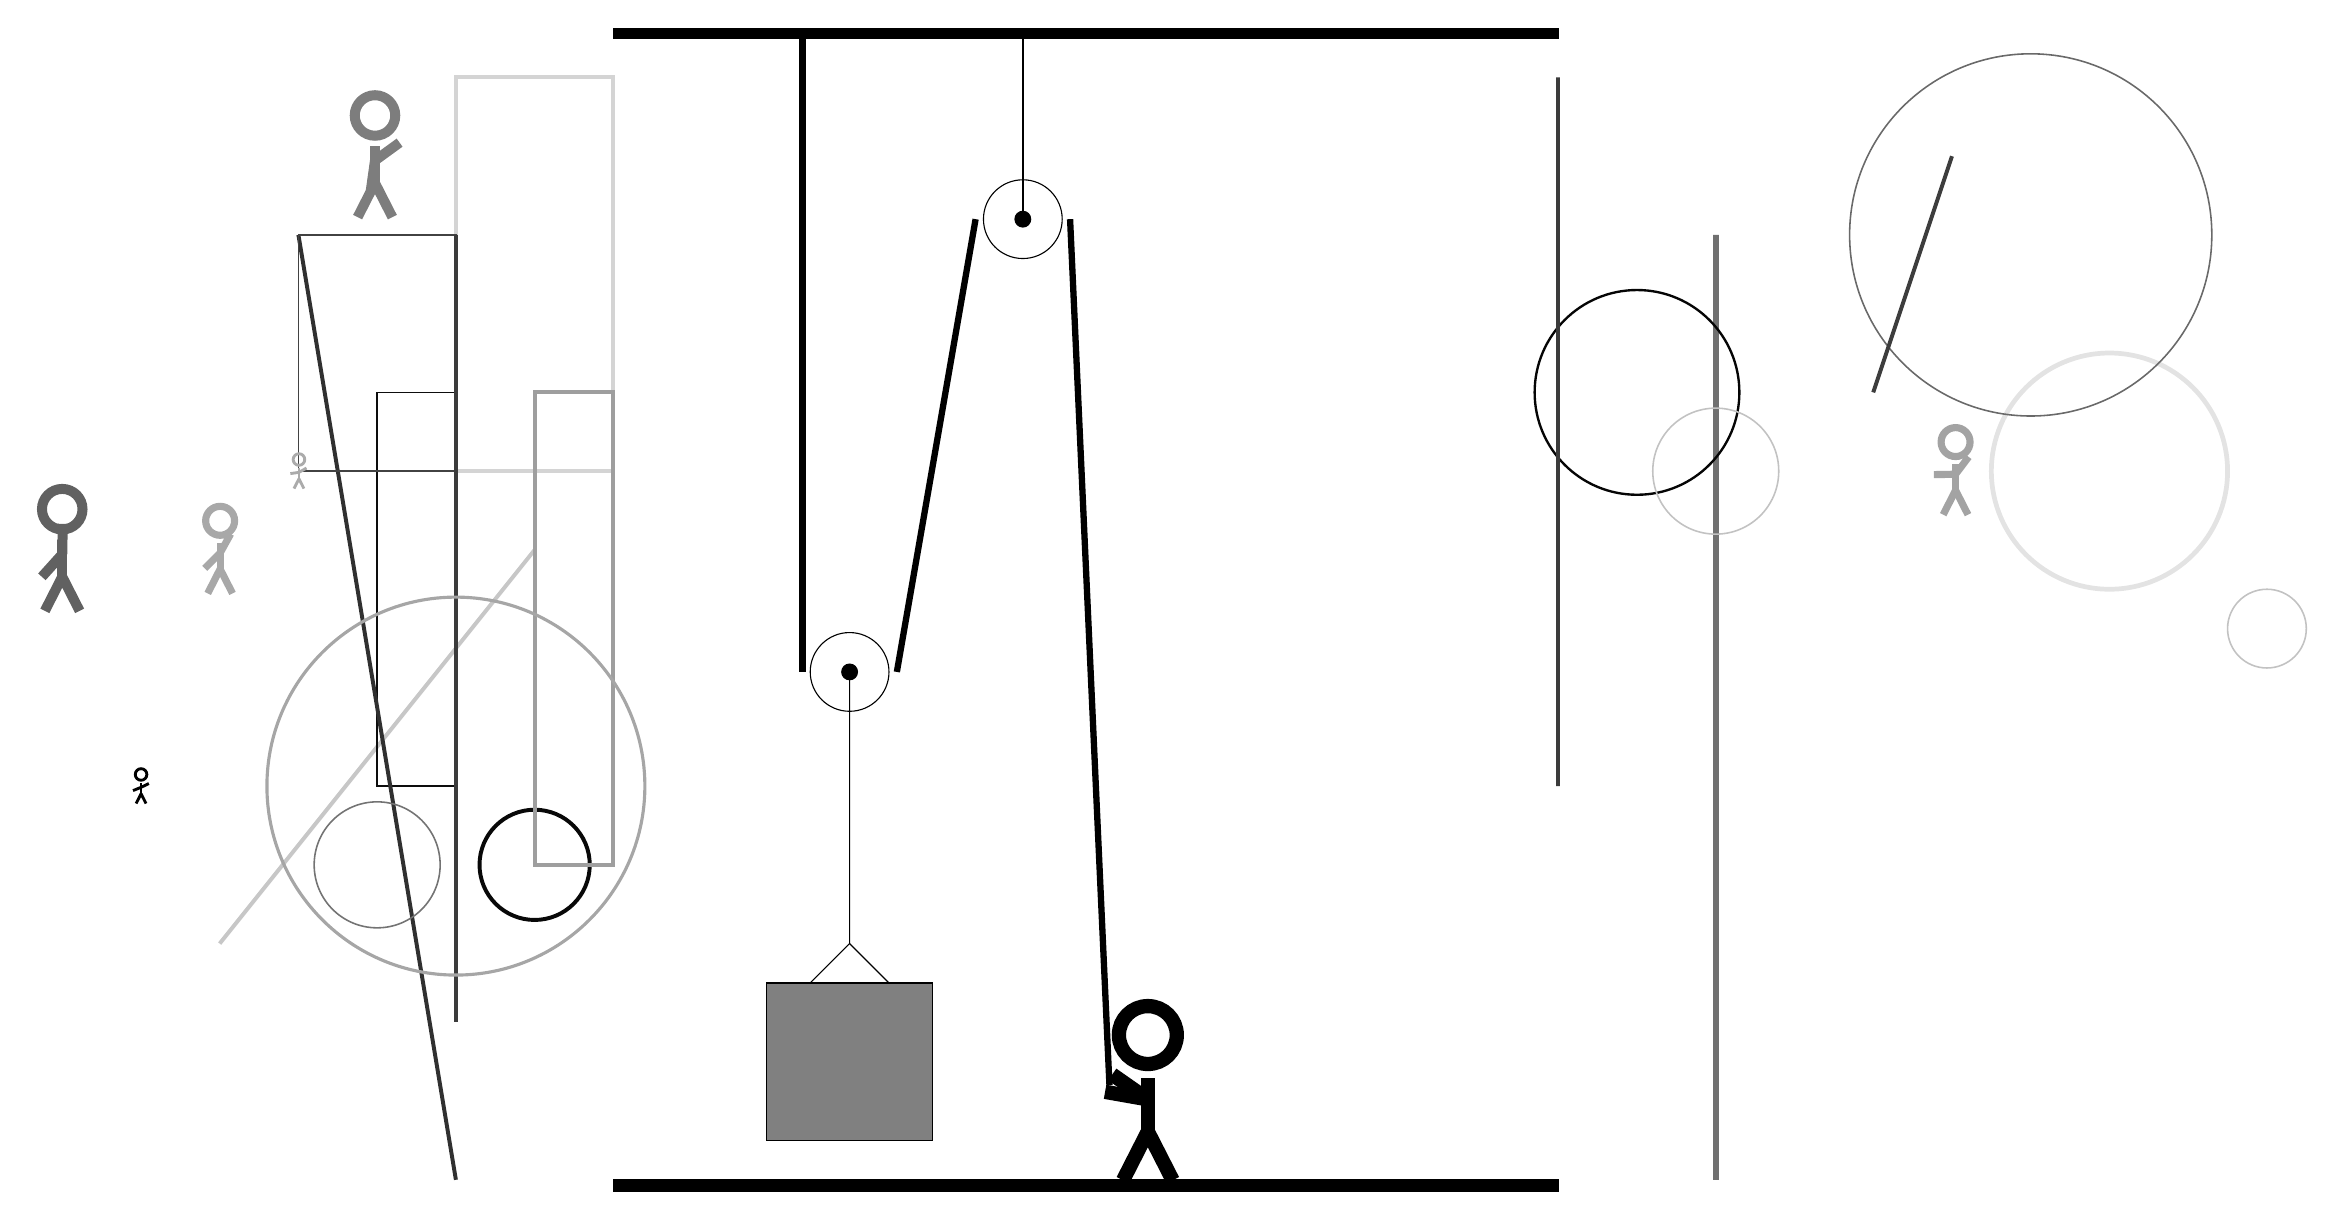
\begin{tikzpicture}
			%%%%% START %%%%%
			
			\draw[fill=black] (-2, 11.5) rectangle (10, 11.625);
			
			\draw (3.2, 9.2) circle (0.5);
			\draw[fill=black] (3.2, 9.2) circle (0.1);
			\draw[thick] (3.2, 9.2) -- (3.2, 11.5);
			
			\draw (1, 3.45) circle (0.5);
			\draw[fill=black] (1, 3.45) circle (0.1);
			
			\draw (1, 3.45) -- (1, 0.0) -- (0.5, -0.5);
			\draw (1, 0.0) -- (1.5, -0.5);
			\draw[fill=black!50] (-0.05, -0.5) rectangle (2.05, -2.5);
			
			\draw[line width=0.8mm] (0.4, 11.5) -- (0.4, 3.45);
			\centerarc[line width=0.8mm](1, 3.45)(180:360:0.6);
			\draw[line width=0.8mm](1.6, 3.45) -- (2.6, 9.2);
			\centerarc[line width=0.8mm](3.2, 9.2)(0:180:0.6);
			\draw[line width=0.8mm](3.8, 9.2) -- (4.3, -1.8);
			
			\node[line width=0.3mm, color=black!100] at (-8, 2) {\Strichmaxerl[2][22][26]};
			
			\draw[line width=0.7mm, color=black!56] (12, 9) rectangle (12, -3);
			\draw[line width=0.5mm, color=black!22](-3, 5) -- (-7, 0);
			\draw [line width=0.5mm, color=black!97](-3, 1) circle (0.7);
			\draw[line width=0.2mm, color=black!95] (-4, 2) rectangle (-5, 7);
			\draw [line width=0.3mm, color=black!98](11, 7) circle (1.3);
			\node[line width=0.3mm, color=black!36] at (15, 6) {\Strichmaxerl[5][1][53]};
			\draw [line width=0.6mm, color=black!11](17, 6) circle (1.5);
			\draw[line width=0.5mm, color=black!81](-4, -3) -- (-6, 9);
			
			\draw[line width=0.5mm, color=black!17] (-4, 6) rectangle (-2, 11);
			\draw[line width=0.2mm, color=black!74] (-4, 9) rectangle (-6, 6);
			\draw[line width=0.5mm, color=black!77](-4, 9) -- (-4, -1);
			\draw[line width=0.5mm, color=black!38] (-3, 7) rectangle (-2, 1);
			\draw [line width=0.2mm, color=black!24](19, 4) circle (0.5);
			\draw [line width=0.3mm, color=black!47](13, 0) circle (0.0);
			\draw [line width=0.2mm, color=black!59](16, 9) circle (2.3);
			\draw [line width=0.5mm, color=black!32](15, -1) circle (0.0);
			\draw[line width=0.5mm, color=black!76](15, 10) -- (14, 7);
			\node[line width=0.6mm, color=black!33] at (-6, 6) {\Strichmaxerl[2][8][30]};
			\draw [line width=0.4mm, color=black!35](-4, 2) circle (2.4);
			\node[line width=0.2mm, color=black!62] at (-9, 5) {\Strichmaxerl[7][48][89]};
			
			\draw [line width=0.2mm, color=black!55](-5, 1) circle (0.8);
			
			\node[line width=0.7mm, color=black!34] at (-7, 5) {\Strichmaxerl[5][45][61]};
			\draw [line width=0.2mm, color=black!24](12, 6) circle (0.8);
			\draw[line width=0.5mm, color=black!77] (10, 11) rectangle (10, 2);
			
			\node[line width=0.6mm, color=black!51] at (-5, 10) {\Strichmaxerl[7][82][36]};
			
			
			\node at (4.7, -1.9) {\Strichmaxerl[10][-35][170]};
			
			\draw[fill=black] (-2, -3) rectangle (10, -3.15);
			
			%%%%% END %%%%%
		\end{tikzpicture}
	\end{figure}	
\end{document}